% F4 — Drift-to-retrain feedback loop
% Standalone TikZ figure: compile with lualatex or pdflatex.
% The enclosing chapter supplies \caption{}; no caption text lives here.
%
% Node identities verified against:
%   src/schedules/src/schedules/drift.py
%   src/schedules/src/schedules/retrain.py
\documentclass[tikz,border=10pt]{standalone}
\usetikzlibrary{positioning, arrows.meta, shapes.geometric, shapes.symbols, calc}

\begin{document}
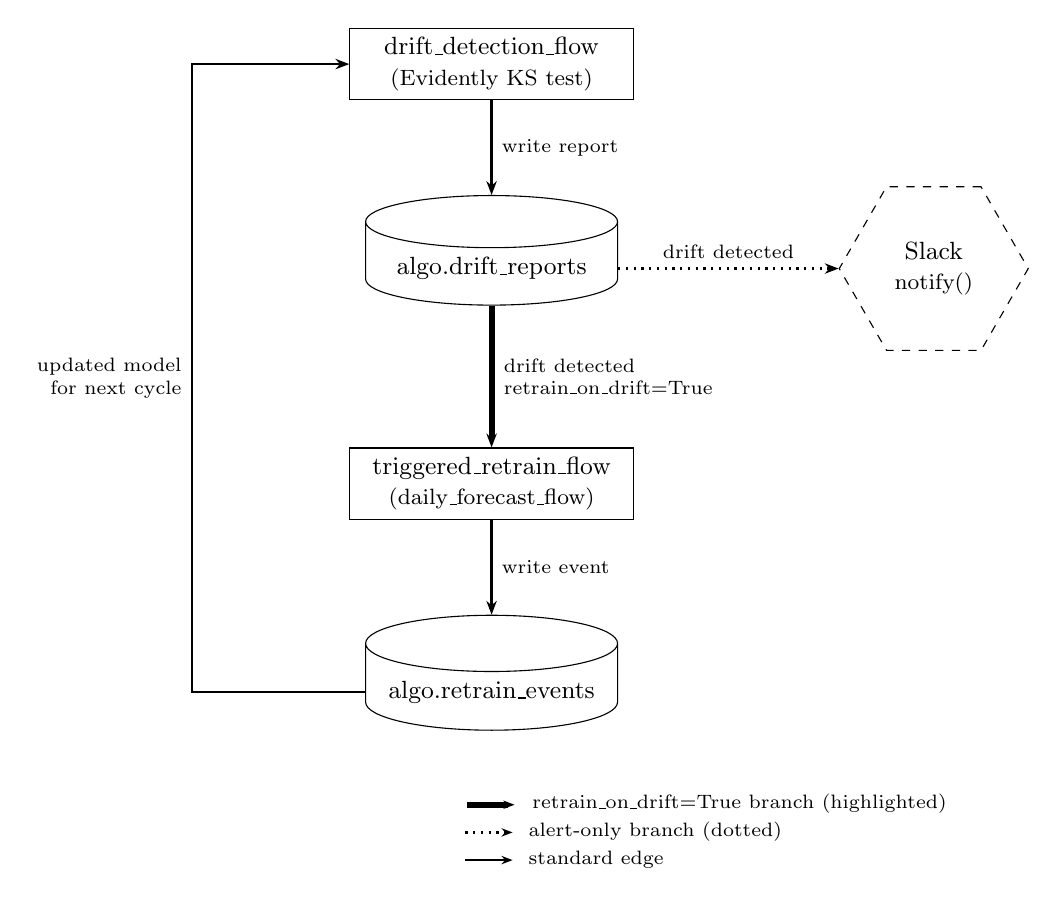
\begin{tikzpicture}[
  % --- node styles ---
  flowbox/.style={
    draw, rectangle,
    minimum width=3.6cm, minimum height=0.9cm,
    align=center, font=\small
  },
  dbcyl/.style={
    draw, cylinder,
    shape border rotate=90,
    minimum width=3.2cm, minimum height=0.75cm,
    align=center, font=\small,
    aspect=0.25
  },
  slackhex/.style={
    draw, regular polygon, regular polygon sides=6,
    minimum width=2.4cm,
    align=center, font=\small,
    dashed
  },
  % --- arrow styles ---
  arr/.style={-{Stealth[length=5pt]}, thick},
  retrain_arr/.style={-{Stealth[length=5pt]}, line width=2.2pt},
  alert_arr/.style={-{Stealth[length=5pt]}, thick, dotted},
]

% ============================================================
% NODES
% ============================================================

% 1. Top: drift detection flow
\node[flowbox] (drift_flow)
    at (0, 0)
    {drift\_detection\_flow\\{\footnotesize (Evidently KS test)}};

% 2. Drift results table (below the flow)
\node[dbcyl] (drift_reports)
    [below=1.2cm of drift_flow]
    {algo.drift\_reports};

% 3. Slack alert (to the right, alert-only branch)
\node[slackhex] (slack)
    [right=2.8cm of drift_reports]
    {Slack\\{\footnotesize notify()}};

% 4. Retrain flow (below drift_reports, retrain_on_drift=True branch)
\node[flowbox] (retrain_flow)
    [below=1.8cm of drift_reports]
    {triggered\_retrain\_flow\\{\footnotesize (daily\_forecast\_flow)}};

% 5. Retrain audit table (below the retrain flow)
\node[dbcyl] (retrain_events)
    [below=1.2cm of retrain_flow]
    {algo.retrain\_events};

% ============================================================
% ARROWS
% ============================================================

% drift_detection_flow → algo.drift_reports (always written)
\draw[arr] (drift_flow.south)
    -- node[right, font=\scriptsize] {write report}
    (drift_reports.north);

% algo.drift_reports → Slack (dotted alert-only branch, drift detected)
\draw[alert_arr] (drift_reports.east)
    -- node[above, font=\scriptsize] {drift detected}
    (slack.west);

% algo.drift_reports → triggered_retrain_flow (thick, retrain_on_drift=True)
\draw[retrain_arr] (drift_reports.south)
    -- node[right, font=\scriptsize, align=left]
        {drift detected\\retrain\_on\_drift=True}
    (retrain_flow.north);

% triggered_retrain_flow → algo.retrain_events (always written)
\draw[arr] (retrain_flow.south)
    -- node[right, font=\scriptsize] {write event}
    (retrain_events.north);

% algo.retrain_events feedback arc back to drift_detection_flow
% (loop: retrain completion feeds back into model used by next drift run)
\draw[arr]
    (retrain_events.west)
    -- ++(-2.2, 0)
    |- node[pos=0.25, left, font=\scriptsize, align=right]
        {updated model\\for next cycle}
    (drift_flow.west);

% ============================================================
% LEGEND
% ============================================================

\node[draw=none, align=left, font=\scriptsize,
      anchor=north west]
    at ($(retrain_events.south west) + (-0.0, -0.7)$) {
    \tikz\draw[retrain_arr, -{Stealth[length=4pt]}] (0,0) -- (0.6,0);
    \ retrain\_on\_drift=True branch (highlighted)\\[2pt]
    \tikz\draw[alert_arr, -{Stealth[length=4pt]}] (0,0) -- (0.6,0);
    \ alert-only branch (dotted)\\[2pt]
    \tikz\draw[arr, -{Stealth[length=4pt]}] (0,0) -- (0.6,0);
    \ standard edge
};

\end{tikzpicture}
\end{document}
